% !TeX root = ../../../main.tex

%************************************************
\section{A positive factorization scheme}
\label{sec:pos/scheme}
%************************************************

We will now construct a positive factorization scheme based on the POS 
subtraction of
Eqs.~(\ref{eq:pos/counthqq}-\ref{eq:counthqg},\ref{eq:counthgg}-\ref{eq:counthgq}).
We then discuss the scheme transformation from this scheme to the
\msbar{} scheme and use it to show that PDFs are non-negative in the
\msbar{} scheme in the perturbative region.

The argument is based on the factorization
Eqs.~(\ref{eq:pos/refaca}-\ref{eq:refacb}), and, very crudely speaking, amounts to
showing that with the POS subtraction, all factors in Eqs.~(\ref{eq:pos/refacb})
are positive: the left-hand side is positive because it is a physically
measurable cross-section, the coefficient $C^S$ function on the right-hand side
is positive because the POS subtraction preserves the positivity of the
unsubtracted coefficient function $C$, which is a partonic cross-section, and
thus positive before subtraction, but only well-defined in $d>4$ dimensions.

Taking a Mellin transform of both sides of
Eqs.~(\ref{eq:pos/refaca}-\ref{eq:refacb}) all convolutions turn into
ordinary products, and it is immediately clear that, because the left-hand
side is positive, for the
Mellin transformed PDF to be positive it is necessary and sufficient
that the coefficient  function is positive. However, 
positivity of the Mellin transform of a function is a necessary
condition for its positivity, but not a sufficient one: a negative
function may have a positive Mellin transform. The somewhat more
complex structure of the discussion below is necessary in order
to deal with the necessity of providing an $x$-space argument.


\subsection{Positive PDFs}
\label{sec:pospdf}

We start by presenting the construction in a simplified setting, 
namely in the absence of parton mixing. This means that the operators
Eq.~(\ref{eq:pos/quark}) whose matrix elements define the PDFs renormalize
multiplicatively.
This would specifically correspond to
the case of a quark combination that does not mix with the
gluon, such as  any combination $q^{\NS}(Q^2)=q_i(Q^2)-q_j(Q^2)$,
where $i,\>j$ denote generically a quark flavor or antiflavor, with
$i\not= j$.  We refer to this as a 
nonsinglet quark combination. We can think of the argument below as
applying to such a combination, 
chosen in such a way that  the bare
$q^{\NS}(Q^2)^{(0)}$, Eq.~(\ref{eq:pos/quark}), is positive --- which in
general of course will not be true even if $q_i$ and $q_j$ are
separately positive. 
This should be viewed as an academic case --- after
all, in principle, a positive nonsinglet PDF might not exist --- whose
purpose is to illustrate the structure of the argument in the absence
of parton mixing. We then turn
to the realistic case of PDFs that do undergo mixing upon
renormalization (which we will refer to as singlet case).
The nonsinglet case is simpler, not only because of the absence of
mixing, but also because in  this case
the POS scheme actually coincides with \msbar{} (i.e., \msbar{} is already
positive). 

\subsubsection{The nonsinglet case as a toy model}
\label{sec:nonsing}

In the nonsinglet case, only the diagonal quark subtraction is relevant: so in
the nonsinglet case the DIS structure function Eq.~(\ref{eq:pos/f2}) becomes
\begin{equation}\label{eq:pos/disfact}
 \frac{1}{x} F_2^{\NS}(x,Q^2)= \langle e_i^2\rangle \left[1
 +\frac{\alpha_s}{2\pi}  C^{(1)}_q \otimes \right] q^{\NS}(Q^2) \,,
\end{equation}
where $q^{\NS}$ is a difference of two quark or antiquark PDFs, assumed
positive and
$\langle
e^2_i\rangle=\frac{1}{2} \left(e^2_i+e^2_j\right)$ is the average of
their electric charges. 

The factorization Eqs.~(\ref{eq:pos/refaca}-\ref{eq:refacb}) takes the
form
\begin{align}
  \frac{1}{x} F_2^{\NS}(x,Q^2)&= \langle e_i^2\rangle
\lim_{\epsilon\to
  0^-}\left[1
    +\frac{\alpha_s}{2\pi} C_{q}^{(1)}(Q^2,\epsilon) \otimes \right] 
    \left[{q^{\NS}}\right]^{(0)} \label{eq:pos/dismsbar} \\
&= \langle e_i^2\rangle
\lim_{\epsilon\to
  0^-}\left[1 +\frac{\alpha_s}{2\pi} {C_{q}^{(1)}}^{\mmsbar}(Q^2, \epsilon) \otimes \right]
  \nonumber\\
  &\qquad\qquad\qquad\qquad\qquad
    \times\left[1 +\frac{\alpha_s}{2\pi} \delta^{\mmsbar} (Q^2,\epsilon) \otimes \right]
     \left[{q^{\NS}}\right]^{(0)} \label{eq:pos/dismsbar1} \\
    &=  \langle e_i^2\rangle
\left[1+ \frac{\alpha_s}{2\pi} {\Delta^{(1)}_q}^{\mmsbar}
  +\frac{\alpha_s}{2\pi}    {\bar{C}_{q}^{(1)}{}}^{\mmsbar} \otimes
  \right] 
     \left[{q^{\NS}}\right]^{\mmsbar}(Q^2) \,, \label{eq:pos/dismsbar2}
\end{align}
where $ {C_{q}^{(1)}}^{\mmsbar}$,  ${\overline{C_{q}}^{(1)}}^{\mmsbar}$,
${\Delta^{(1)}_q}^{\mmsbar}$ and $ \delta_{qq}^{\mmsbar} $ have been
defined in Eqs.~(\ref{eq:pos/cqnodist},\ref{eq:cqren},\ref{eq:renormq}),
and the dependence on $x$ on the  right-hand side has been omitted
because it appears due to the convolution, while the dependence on all
other variables has been indicated explicitly.

Now, the discussion of Sect.~\ref{sec:discf} shows that, because the
bare PDF of Eq.~(\ref{eq:pos/quark}) is a probability density, the three
factors which are convoluted in Eq.~(\ref{eq:pos/dismsbar2}) are all
separately positive when $\epsilon \to 0^-$, i.e.\ from the negative
region, provided only $\mu^2< \mu_D^2$, with $\mu_D^2$ given by
Eq.~(\ref{eq:pos/mud})\footnote{Note that the condition cannot be satisfied in
the strict $x\to1$ limit, but this is as it should be since in the
limit the scattering process becomes elastic and it is no longer
described by perturbative QCD.}.
This, as discussed in Sect.~\ref{sec:diag} [see in particular
Eq.~(\ref{eq:pos/cqnlo}) and Fig.~\ref{fig:dis}]
can be understood as a consequence of the fact that the only region in
which the $O(\alpha_s)$ term could overwhelm the LO contribution is
the threshold region $z\to 1$, where $\alpha_s\ln(1-z)\sim1$.
However, in this region the \msbar{} over-subtraction leads to a
coefficient function which is positive because $P_{qq}$ is negative at
large $z$. Consequently, all factors in  Eq.~(\ref{eq:pos/dismsbar2})
remain positive for all $z$.

The  meaning of the factorization argument
Eqs.~(\ref{eq:pos/dismsbar}-\ref{eq:dismsbar2}) can be understood by
noting
that it is possible to choose a ``physical'' factorization
scheme~\cite{Catani:1995ze} in which PDFs are identified with physical
observables. This means that the coefficient function is set to one to
all orders by scheme choice. An example is the ``DIS'' scheme~\cite{Diemoz:1987xu} in which
the quark PDF is identified with the DIS structure function, so that
Eq.~\ref{eq:pos/disfact} becomes
\begin{equation}\label{eq:pos/disfactns}
 \frac{1}{x} F_2^{\NS}(x,Q^2)= \langle e_i^2\rangle  \left[{q^{\NS}}\right]^{\textrm{DIS}}(x,Q^2) \,,
 \end{equation}
which holds to all perturbative orders. Comparing this DIS scheme
expression of the structure function to the \msbar{} expression,
Eq.~(\ref{eq:pos/f2}), immediately shows that the quark PDF in the DIS
and \msbar{} schemes are related by
\begin{equation}\label{eq:pos/msbartodis}
\left[{q^{\NS}}\right]^{\textrm{DIS}}(\xi,Q^2)=
\left[1+\frac{\alpha_s}{2\pi} {\Delta^{(1)}_q}^{\mmsbar}
  +\frac{\alpha_s}{2\pi}
  {{{\bar{C}}^{(1)}}_q{}}^{\mmsbar}\otimes\right]\left[{q^{\NS}}\right]^{\mmsbar}(Q^2) \,,
\end{equation}
where again we have dropped the $\xi$ dependence of the convolution
on the right-hand side,
as in Eqs.~(\ref{eq:pos/dismsbar}-\ref{eq:dismsbar2}).

The \msbar{} PDFs can be obtained in terms of the DIS ones by inverting
Eq.~(\ref{eq:pos/msbartodis}): perturbative inversion of course gives
\begin{equation}\label{eq:pos/distomsbar}
\left[{q^{\NS}}\right]^{\mmsbar}(\xi,Q^2)=
\left[1-\frac{\alpha_s}{2\pi} {\Delta^{(1)}_q}^{\mmsbar}
  -\frac{\alpha_s}{2\pi}  {\bar
    C^{(1)}_q{}}^{\mmsbar}\otimes\right]\left[{q^{\NS}}\right]^{\textrm{DIS}}(Q^2)
+O(\alpha_s^2) \,.
\end{equation}
One may worry that therefore the \msbar{} PDFs may turn negative in the
large $\xi$ region, where $\alpha_s\ln(1-\xi)\gtrsim 1$ and the last term
in square brackets in Eq.~(\ref{eq:pos/distomsbar}), which is negative, may overwhelm the LO
contribution 
term. However, in this region the perturbative
inversion is invalid, but it is easy to invert
Eq.~(\ref{eq:pos/msbartodis}) exactly in the asymptotic large $\xi$ limit.
Letting
\begin{align}\label{eq:pos/msbartodisp}
    \hspace{-20pt}\left[{q^{\NS}}\right]^{\textrm{DIS}}(\xi,Q^2)&=
\left[1+\frac{\alpha_s}{2\pi} {\Delta^{(1)}_q}^{\mmsbar}
  +\frac{\alpha_s}{2\pi} 2C_F\left[\frac{\ln(1-z)}{1-z}\right]_+
  \otimes\right]\left[{q^{\NS}}\right]^{\mmsbar}(Q^2)\nonumber\\
    &\qquad+ \hbox{NLL}(1-\xi)\\
\label{eq:pos/msbartodisp1}
    &= \left(1+\frac{\alpha_s}{2\pi} {\Delta^{(1)}_q}^{\mmsbar}\right) 
\left[1+c_{\textrm{LL}}\left[\frac{\ln(1-z)}{1-z}\right]_+
\otimes\right]\left[{q^{\NS}}\right]^{\mmsbar}(Q^2)\nonumber\\
    &\qquad+ \hbox{NLL}(1-\xi) \,,
\end{align}
with
\begin{equation}
    \label{eq:pos/msbartodiscoeff}
    %\hfill
    c_{\textrm{LL}} = \frac{\frac{\alpha_s}{2\pi} 2C_F}{1+\frac{\alpha_s}{2\pi} {\Delta^{(1)}_q}^{\mmsbar}} \,, 
    %\hfill
\end{equation}
and which holds at the leading $\ln(1-\xi)$ level (LL$(1-\xi)$),
inversion can be performed by going to Mellin space and then computing
the Mellin inverse term by term in an expansion in powers of $\alpha_s$.
We get
\begin{align}\label{eq:pos/distomsbarllx}
    \hspace*{-20pt} \left[{q^{\NS}}\right]^{\mmsbar}(\xi,Q^2) &= \frac{1}{1+\frac{\alpha_s}{2\pi} {\Delta^{(1)}_q}^{\mmsbar}} \times \nonumber\\
    &\hspace*{-60pt}\Bigg[1 -c_{\textrm{LL}} \left[ \frac{\ln(1-z)}{\left[1+c_{\textrm{LL}}\ln^2(1-z)/2\right]^2}  \frac{1}{1-z}\right]_+
\otimes\Bigg]\left[{q^{\NS}}\right]^{\textrm{DIS}}(Q^2) + \hbox{NLL}(1-\xi) \,.
\end{align}
It is clear that as $\xi\to 1$ the negative LL$(1-\xi)$ contribution
actually vanishes.\footnote{A similar argument also applies at small
  $\xi$, where the coefficient function also rises, as seen in
  Fig.~\ref{fig:dis}. We do not discuss this case in detail since
  positivity of the \msbar{} PDF at small $\xi$ is manifest.}




Now, we observe that
$\left[{q^{\NS}}\right]^{\textrm{DIS}}(\xi,Q^2)$ is positive because it is a physical
observable. Equation~(\ref{eq:pos/msbartodis}), which expresses the DIS
PDF in terms of the \msbar{} one, then  implies that  for
$\left[{q^{\NS}}\right]^{\mmsbar}(\xi,Q^2)$  to be guaranteed to be
positive,
the \msbar{} coefficient function  must also be positive, otherwise
folding a positive \msbar{}  PDF with a negative coefficient function
could lead to a negative DIS PDF. So positivity of the \msbar{}
coefficient function
is a necessary condition for positivity of the \msbar{} PDF.
However, the inverse of  Eq.~(\ref{eq:pos/msbartodis}), expressing the
\msbar{} PDF in terms of the DIS one, implies that the condition is
also sufficient, because it gives the \msbar{} PDF as the convolution
of a positive coefficient with a positive PDF. Equations.~(\ref{eq:pos/distomsbar},\ref{eq:distomsbarllx}) show that the coefficient is indeed
positive because in the dangerous
$\xi\to 1$ region, where  a large negative contribution may arise,
inversion can be performed exactly and shown to lead to a positive
result.
Of
course, this argument works for any factorization scheme, and it shows
that a necessary and (perturbatively) sufficient condition for the
PDFs to be positive is that the coefficient function in that scheme is positive.

The perturbative nature of the argument is worth commenting
upon. As discussed at the beginning of this section, the corresponding
Mellin space argument is trivial: because in Mellin space the
structure function is the product of the PDF times the coefficient
function, it follows that positivity of the coefficient function is
necessary and sufficient for the positivity of the PDF. However, as
already mentioned,
Mellin-space positivity is not sufficient for $x$-space positivity. It
is therefore necessary to compute the $x$-space inverse of the
coefficient function, and check that it is still positive.

The
inversion is done perturbatively in Eq.~(\ref{eq:pos/distomsbar}), and it
leads to a coefficient function which is manifestly positive in most
of the $z$ range, except at small and large $z$, where the coefficient
functions blows up, due to high-energy (BFKL) and soft (Sudakov) logs
respectively. Consider the large-$z$ case that was discussed
above. Upon 
Mellin transformation, the $z\to 1$ region is mapped onto the
$N\to\infty$ region, and specifically, as well known (see
e.g. Ref.~\cite{Forte:2002ni}) powers of $\ln(1-z)$ are mapped onto
powers of $\ln N$.  
The $\ln N$ logarithmic growth of the coefficient function in this limit is
seen in Fig.~\ref{fig:dis}, where it is apparent that the coefficient function
diverges as $N\to\infty$. The $N$-space inverse of the coefficient function is
just its reciprocal, and thus it manifestly vanishes as $N\to\infty$ (while of
course remaining positive).
One would therefore naively expect that the $x$-space inverse also vanishes
(from the positive side) as $z\to1$, and this expectation is borne out by the
explicit computation presented above in
Eq.~(\ref{eq:pos/distomsbarllx}).\footnote{
  Since the Mellin space inverse coefficient function behaves as $[\bar
  C^{(1)}(N)]^{-1}\toinf{N}\frac{1}{\ln^2 N}$ it may appear surprising hat the
  term in square brackets in Eq~(\ref{eq:pos/distomsbarllx}) starts with one.
  However, it should be born in mind that the Mellin transform of any function
  which is regular (or indeed integrable) at $x=1$ vanishes as $\frac{1}{N^k}$,
  with $k>0$, hence in Mellin space the suppression of the inverse coefficient
  function as $N\to\infty$ is a subleading correction to the leading power
  suppression of $q^{\textrm{NS}}(N)$.
}
Similar arguments apply at higher orders (NNLO and beyond), where the
coefficient function grows with a higher order power of $\ln(1-z)$ as $z\to1$,
and at small $z$, where the coefficient function grows as powers of $\ln
\frac{1}{z}$ as $z\to0$.
Hence, either the coefficient function is not logarithmically enhanced, and
then the perturbative inverse is manifestly positive, or it is logarithmically
enhanced, and then the exact inverse of the enhanced terms can be computed ans
also shown to be positive.
It is natural to conjecture that an explicit computation of the exact inverse
of the full coefficient function would also be positive.

The perturbative  assumption is therefore used in two different
ways. On the one hand, the NLO correction to the \msbar{}  coefficient function
 ${\bar  C^{(1)}_q(z)}^{\mmsbar}$ is not everywhere positive, as it is
apparent from Fig.~\ref{fig:dis}. However, this is a small correction
to the positive coefficient function if $\alpha_s\lesssim 1$, and the
overall coefficient function remain positive. This would fail in a
region in which $\alpha_s$ blows up. So the full NLO coefficient
function remains positive, but only in the perturbative region. On the other
hand, the perturbative inversion Eq.~(\ref{eq:pos/distomsbar}) is used to
show that positivity of the coefficient function is shared by its
inverse, and in regions in which perturbativity would fail it is
checked explicitly that this is the case by exact inversion. In this
case we conjecture that positivity of the inverse is actually an exact
property, even when $\alpha_s$ is arbitrarily large.

The argument based on the physical factorization scheme showing that
a positive coefficient function is necessary and (perturbatively)
sufficient for a positive PDF is in fact equivalent to the
factorization argument
Eqs.~(\ref{eq:pos/dismsbar}-\ref{eq:dismsbar2}). Indeed, 
the operator definition of the quark distribution, Eq.~(\ref{eq:pos/quark}),
upon performing a derivative expansion of the Wilson line, leads to
the standard expression of its moments in terms of matrix elements of
local operators. The interpretation of the bare quark distribution as
a probability  is then
preserved by any physical subtraction scheme such that the matrix
elements of Wilson operators are expressed in terms of a measurable
quantity. The DIS scheme of Eq.~(\ref{eq:pos/disfact}) is of course an
example of this scheme. Given the equivalence of the two arguments,
one may wonder whether, if at all, perturbativity is used in the
argument of Eqs.~(\ref{eq:pos/dismsbar}-\ref{eq:dismsbar2}): specifically,
the perturbative inversion of Eq.~(\ref{eq:pos/distomsbar}). The question is
answered in the affirmative: the perturbative inversion is hidden in the step leading from Eq.~(\ref{eq:pos/dismsbar})
to Eq.~(\ref{eq:pos/dismsbar1}). Indeed, this step amounts to 
\begin{equation}\label{eq:pos/exinv}
\left[1
  +\frac{\alpha_s}{2\pi} {C_{q}^{(1)}}^{\mmsbar}\otimes\right]^{-1} \left[1
    +\frac{\alpha_s}{2\pi} C_{q}^{(1)}(Q^2,\epsilon)\right]=
\left[1
    +\frac{\alpha_s}{2\pi} \delta^{\mmsbar} (Q^2,\epsilon)\right]
+O(\alpha_s^2) \,,
\end{equation}
i.e.\ the perturbative inversion of the \msbar{} coefficient function. 
The two arguments are thus seen
to coincide. Again, while we only provide a perturbative argument it
is natural to conjecture that the argument is in fact exact (i.e.\ it
also holds for large values of $\alpha_s$).
 


\subsubsection{The POS factorization scheme}
\label{sec:pos}

Equipped with the results of Sect.~\ref{sec:nonsing} we can  turn to
the case in which parton mixing is present.   This corresponds to the
realistic case in which the operators Eq.~(\ref{eq:pos/quark}) mix with
the gluon and conversely (at NLO) and with each other at NNLO and
beyond. Because at NLO only quark-gluon mixing is present, we refer to
this as the singlet case.
In order to fully define
the factorization scheme at NLO we must thus consider a pair of
processes, a quark-induced and a gluon-induced one.
The factorization for a pair of hadronic processes
can be written as 
\begin{equation}\label{eq:pos/singhadfact}
 \frac{1}{x} \sigma(x,Q^2)= \hat \Sigma_0\otimes \left[1
 +\frac{\alpha_s}{2\pi}  C^{(1)} \otimes \right] f(Q^2) \,.
 \end{equation}
In Eq.~(\ref{eq:pos/singhadfact}) \begin{itemize}
  \item $\sigma(x,Q^2)$ is a vector of hadronic cross sections
\begin{equation}\label{eq:pos/hadxsec}
   \sigma(x,Q^2)=\left(\begin{array}{c} \sigma^{q}(x,Q^2)\\ \sigma^{g} (x,Q^2)\end{array}\right),
\end{equation}
 such as
the pair of processes of Sect.~\ref{sec:hadr}, namely Drell--Yan  and
Higgs production in gluon fusion; we are assuming for simplicity  and without loss of
generality that both are evaluated at the same scale $Q^2=M^2$ (such
as when producing an off-shell gauge boson and/or Higgs with the same
mass), with a trivial generalization to the case of unequal scales,
and the scaling variable is $x=\frac{Q^2}{s}$, with $s$ the hadronic
center-of-mass energy;
\item $\hat \Sigma_0$ is a diagonal matrix of LO partonic cross sections,
  multiplied by the respective PDFs, 
\begin{equation}\label{eq:pos/lohadxsec}
   \hat \Sigma_0(x,Q^2)=\left(\begin{array}{cc} \hat \sigma_0^{q} q (x,Q^2) &
   0 \\0 & \sigma_0^{g} g (x,Q^2) \end{array}\right),
\end{equation}
namely the quark and the gluon respectively for Drell--Yan and Higgs;
\item $C^{(1)}$ is the two-by-two matrix of NLO 
  coefficient functions ${C^i{}_{j}}^{(1)}$ with $i,\, j=q,\, g$
  defined in Eq.~(\ref{eq:pos/hadfact});
\item $f(\xi,Q^2)$ is a vector of PDFs that mix upon renormalization:
\begin{equation}\label{eq:pos/singpdf}
   f(\xi,Q^2)=\left(\begin{array}{c} q(\xi,Q^2) \\ g(\xi,Q^2) \end{array}\right).
\end{equation}
\end{itemize}

Having established a suitable notation, the argument then proceeds
in an analogous way as the nonsinglet argument of
Sect.~\ref{sec:nonsing}, except that now, in order to guarantee
positivity of the two-by-two matrix of coefficient functions, we must
perform the POS subtraction, which in the diagonal
channels (and thus in the nonsinglet case) coincides with \msbar{} but
in the off-diagonal channel differs from it.
Namely, we have
\begin{align}
\frac{1}{x} \sigma(x,Q^2)&= \hat \Sigma_0\otimes
\lim_{\epsilon\to
  0^-}\left[\mathbb{I}
    +\frac{\alpha_s}{2\pi} C^{(1)}(Q^2,\epsilon) \otimes\right]
    f^{(0)} \label{eq:pos/posmsbar} \\
&= \hat \Sigma_0\otimes
\lim_{\epsilon\to
  0^-}\left[\mathbb{I}
  +\frac{\alpha_s}{2\pi} {C^{(1)}}^{{\textrm{POS}}}(Q^2,\epsilon) \otimes\right]
\left[\mathbb{I}
    +\frac{\alpha_s}{2\pi} \delta^{{\textrm{POS}}} (Q^2,\epsilon)\otimes\right]
    f^{(0)} \label{eq:pos/posmsbar1} \\
    &=  \hat \Sigma_0\otimes
\left[\mathbb{I}+ \frac{\alpha_s}{2\pi} {\Delta^{(1)}}^{{\textrm{POS}}}
  +\frac{\alpha_s}{2\pi}    {\overline{C}^{(1)}}^{{\textrm{POS}}} \otimes
  \right] 
     f^{{\textrm{POS}}}(Q^2) \,. \label{eq:pos/posmsbar2}
\end{align}
In Eqs.~(\ref{eq:pos/posmsbar}-\ref{eq:posmsbar2})\begin{itemize}
\item $ {\Delta^{(1)}}^{{\textrm{POS}}}$ is the diagonal matrix
\begin{equation}\label{eq:pos/Deltamat}
  {\Delta^{(1)}}^{{\textrm{POS}}}=\left(\begin{array}{cc} {\Delta_{qq}^{(1)}}^{\mmsbar} &
   0 \\0 & {\Delta_{gg}^{(1)}}^{\mmsbar} \end{array}\right),
\end{equation}
with  ${\Delta_{ii}^{(1)}}^{\mmsbar}$ defined in Eqs.~(\ref{eq:pos/dyq}) and
(\ref{eq:pos/higgsg}) respectively for $i=q$ and $i=g$;
\item $\delta^{{\textrm{POS}}} (Q^2,\epsilon)$ is a two-by-two matrix of
  counterterms
\begin{equation}\label{eq:pos/deltamat}
 \hspace*{-3em}\delta^{{\textrm{POS}}} (z,Q^2,\epsilon)= \left(-\frac 1
    {\epsilon}+\gamma_E\right) \left(\begin{array}{cc}  \left(\frac{Q^2}{4\pi
      \mu^2}\right)^{-\epsilon} P_{qq}(z) & \frac{1}{1-\epsilon}\left(\frac{\mu_h^2}{\pi\mu^2}\right)^{-\epsilon} 
  P_{qg}(z)   \\\frac{1}{1-\epsilon}\left(\frac{\mu_h^2}{\pi\mu^2}\right)^{-\epsilon} P_{gq}(z)  & \left(\frac{Q^2}{4\pi
      \mu^2}\right)^{-\epsilon} P_{gg}(z)  \end{array}\right),
\end{equation}
with $\mu_h^2$ given by  Eq.~(\ref{eq:pos/ktmaxh}), so that in the
diagonal channels the subtraction is the same as in \msbar{}, while in
the off-diagonal channels it is performed at the physical scale
$\mu_h^2$, and also, accounting for the $d$-dimensional continuation of
the  average over the polarization of the gluons.
  \end{itemize}

Positivity of the quark and gluon PDF vector $ f^{{\textrm{POS}}}(Q^2)$,
Eq.~(\ref{eq:pos/posmsbar2}), now follows from the same argument used to
show the positivity of the nonsinglet PDF 
Eq.~(\ref{eq:pos/dismsbar2}). Namely, all
factors, which are convoluted in Eq.~(\ref{eq:pos/dismsbar2}), are 
separately positive when $\epsilon \to 0^-$ and  $\mu_h^2 < \mu_D^2$ (with
$\mu_D$ defined in Eq.~(\ref{eq:pos/mud})) and in particular, the matrix of POS-scheme coefficient
functions is now positive as shown in Sect.~\ref{sec:hadr}.

Also, as in the nonsinglet case,  the positivity argument can be formulated in terms of
a physical scheme, in which now 
to all perturbative orders the quark and gluon are defined by
\begin{equation}\label{eq:pos/phys}
 \frac{1}{x} \bar\sigma(x,Q^2)=f^{\textrm{PHYS}}(x,Q^2) \,,
\end{equation}
where, as in Ref.~\cite{Altarelli:1998gn}, the hadronic cross sections $\bar\sigma(x,Q^2)$ are computed
assuming that one of the two incoming protons is replaced 
by a beam of antiquarks or a beam of gluons respectively, i.e.\ 
\begin{equation}\label{eq:pos/physxsec}
   \bar\sigma(x,Q^2)=\left(\begin{array}{c} \sigma(x,Q^2)[\bar q
       p\to \gamma^*+X]\\ \sigma(x,Q^2)[gp \to H+X]\end{array}\right).
\end{equation}
This hadronic cross section is linear in the PDFs, it coincides with it
at LO in any scheme, and, assuming that it coincides with it to all
orders, defines the PHYS scheme. Equivalently, one could choose as
$\bar \sigma$ a DIS structure function in the quark channel, and the
cross section for Higgs production in photon-gluon fusion in the gluon
channel.
The POS and PHYS schemes are then related by
\begin{equation}\label{eq:pos/postodis}
f^{\textrm{PHYS}}(x,Q^2)=
\left[\mathbb{I}+\frac{\alpha_s}{2\pi} {\Delta^{(1)}}^{\textrm{POS}}
  +\frac{\alpha_s}{2\pi}  {\bar
    C^{(1)}{}}^{\textrm{POS}}\otimes\right]f^{\textrm{POS}}(Q^2) \,,
\end{equation}
which is perturbatively inverted as  
\begin{equation}\label{eq:pos/distopos}
f^{\textrm{POS}}(x,Q^2)=
\left[\mathbb{I}-\frac{\alpha_s}{2\pi} {\Delta^{(1)}}^{\textrm{POS}}
  -\frac{\alpha_s}{2\pi}  {\bar
    C^{(1)}{}}^{\textrm{POS}}\otimes\right]f^{\textrm{PHYS}}(Q^2)+O(\alpha_s^2)\,.
\end{equation}

Again, this shows that positivity of the POS-scheme  coefficient function is
necessary for positivity of the POS-scheme PDFs and sufficient if
perturbativity holds. Just like in the case of
Eq.~(\ref{eq:pos/distomsbar}), this assumption fails at the endpoints
$z\to0$ and $z\to 1$. However, as well known~\cite{Ellis:1991qj}, and
as it is easy to check from the explicit expressions of the matrix
elements of ${\bar
    C^{(1)}(z)}^{\textrm{POS}}$, in both these limits the matrix
  is diagonal up to power-suppressed corrections. Specifically, 
 in the $z\to1$ limit the coefficient function matrix is diagonal:
\begin{equation}\label{eq:pos/diag}
    \lim_{z\to 1}  {C^{(1)}}^{\textrm{POS}}(z,Q^2)=\left(\begin{array}{cc} {{{C^{q}}_q}^{(1)}}^{\textrm{POS}} &
      0 \\0 & {{{C^{g}}_g}^{(1)}}^{\textrm{POS}} \end{array}\right)\left[1+O(1-z)\right].
\end{equation}
Indeed, diagonal coefficient functions grow as
$\left(\frac{\ln(1-z)}{(1-z)}\right)_+$ while off-diagonal ones tend to a constant
as $z\to1$. This is clearly seen in the $N$ space plots of
Figs.~\ref{fig:dy}-\ref{fig:higgs}, in which as $N\to\infty$ the diagonal coefficient
functions are seen to grow (as $\ln^2N$) while the off-diagonal ones
vanish (as $\frac{1}{N}$)~\footnote{The same power behavior also
  holds in the \msbar{} scheme, where however the off-diagonal
  coefficient functions grow as $\ln(1-z)$ as $z\to 1$, corresponding
  to a $\frac{\ln N}{N}$ behavior of its Mellin transform at large $N$.}
It follows that at large $z$ the quark and gluon channels decouple, and
the perturbativity argument is the same as in the
nonsinglet case. 

\subsubsection{Positive PDFs and their scale dependence}
\label{sec:ap}


In Section~\ref{sec:pos}
we have shown that also in the presence of quark-gluon
mixing  POS-scheme
coefficient functions are positive, and thus in the perturbative
regime PDFs are also positive. One can then ask two (closely related)
questions. First, at which scale does this conclusion apply, and is it
affected by perturbative evolution? And second, which PDF combinations
are actually positive?
Indeed, as well known, the eigenstates of QCD evolution are the two
eigenstates of a mixing matrix between the quark singlet and the
gluon,  and individual nonsinglet components; any PDF (and thus any
observable) can be decomposed into a singlet and nonsinglet component,
which evolve independently (see
e.g.\ Sect.~4.3.3 of Ref.~\cite{Ellis:1991qj}). Of course a difference
between two positive quantities is not necessarily positive, so this
raises the question of which are actually the positive combinations:
the eigenstates of evolution, or individual quark, antiquark and
gluons (or indeed something else)?

In order to answer the questions, we start from the observation that
the operators whose matrix elements separately define probability densities are
the quark operators Eq.(\ref{eq:pos/quark}), and their antiquark and gluon
counterparts. This can be understood physically in a simple way by
considering a moment of the PDF: for example, the second moment of the
PDF for quark of flavor $i$ is just the matrix element of the energy
(Hamiltonian) operator for the corresponding quark, expressed in terms
of creation and annihilation operators for the given quark state.
Ditto for each antiquark of
flavor $j$, and for the gluon. Hence, at leading order the quantities
which are separately positive are individual quark flavors, antiquark
flavors, and the gluon.

The argument presented in Section~\ref{sec:pos} shows that this
positivity is preserved for the quark and gluon PDF, which at this
order mix to first order in $\alpha_s$. This argument does not make
any assumption about the particular value of $Q^2$, except that it
ought to be in the perturbative region where $\alpha_s(Q^2)$ is small
enough. Hence, positivity must necessarily be preserved by QCD
evolution.

Actually,  that this is the case directly follows from the construction of the
positive subtraction scheme.
Indeed, QCD evolution of the PDF is a consequence of the $Q^2$
dependence induced by the factorization into the PDF of
scale-dependent collinear logs, i.e., by the scale dependence of the
renormalization factor $Z^S_{ij}(Q^2)$ in
Eqs.~(\ref{eq:pos/pdffac},\ref{eq:pertz}). Indeed, using in these
equations
the explicit form
of the subtraction, as given in
Eqs.~(\ref{eq:pos/cgren},\ref{eq:cqren},\ref{eq:cgqren}) it follows that
upon a change of the scale at which the subtraction is performed, the
renormalization factor changes according to
\begin{equation}\label{eq:pos/dglap}
  Z^S_{ij}({Q'}^2)=\left(\delta_{ij}+\frac{\alpha_s({Q'}^2)}{2\pi}P_{ij}\ln\frac{{Q'}^2}{Q^2}\right)\otimes
  Z_j(Q^2) +O(\alpha_s^2),
\end{equation}
where $P_{ij}$ is the Altarelli-Parisi splitting function. Of course,
taken in differential form for infinitesimal scale changes
Eq.~(\ref{eq:pos/dglap}) is the standard QCD evolution equation.

The POS factorization scheme construction essentially amounts to
choosing $\delta^{S}_{ij}$ in Eq.~(\ref{eq:pos/pertz}) in  such a way that
$Z_{ij}^{S}$ remains positive for all $Q^2$: in particular, whenever
$P_{ij}$ is negative, this will mean that as the scale is increased,
the renormalization factor $Z_{ij}^S$ decreases, while (in a positive
scheme) remaining positive. Clearly, the condition is more easily
satisfied at higher scales because of asymptotic freedom, in agreement
with the phenomenological observation~\cite{Ball:2010de,Ball:2014uwa}
that positivity constraints are more restrictive if imposed at low
scale and are preserved by evolution.

It is worth noting that a consequence of Eq.~(\ref{eq:pos/dglap}) is that,
as well known, a scheme change will affect the NLO splitting
functions. In particular, in the POS scheme contributions proportional
to $\ln\frac{(1-z)^2}{z}$ to the off-diagonal splitting function will
now be automatically resummed to all orders when solving the NLO QCD
evolution equations. These contributions are actually power-suppressed
as $z\to1$, so this resummation is likely not to have a significant
effect: the POS scheme is thus useful as a means to obtain positive
PDFs (which is our main goal here), but not necessarily
phenomenologically better than the standard \msbar{} scheme. On the
other hand, in Ref.~\cite{Jadach:2016acv} a factorization scheme has
been advocated, called the Monte Carlo scheme, that is similar in
spirit to the POS scheme in the off-diagonal channel, but also
modifies the \msbar{} subtraction in the diagonal channel by an
analogous change of subtraction point. In this Monte Carlo scheme,
$\ln(1-z)^2$ contributions in the diagonal channels are also resummed
when solving the QCD evolution equation: hence, leading-log threshold (Sudakov)
resummation is automatically performed, without having to be added a
posteriori. It can be argued that in this Monte Carlo scheme PDFs also
resepect positivity~\cite{jadprivate}.



\subsection{Positive schemes vs.\ \msbar{}}
\label{sec:gen}

In the previous section, we have shown that coefficient functions and
PDFs in the POS
factorization scheme are indeed positive. We would like now to
investigate the relation of the POS scheme to other factorization
schemes, specifically \msbar{}, and the related issue 
of
how a positive factorization scheme should be and can be defined.

\subsubsection{General positive schemes}
\label{sec:gensch}


\begin{figure}[t]
  \begin{center}
    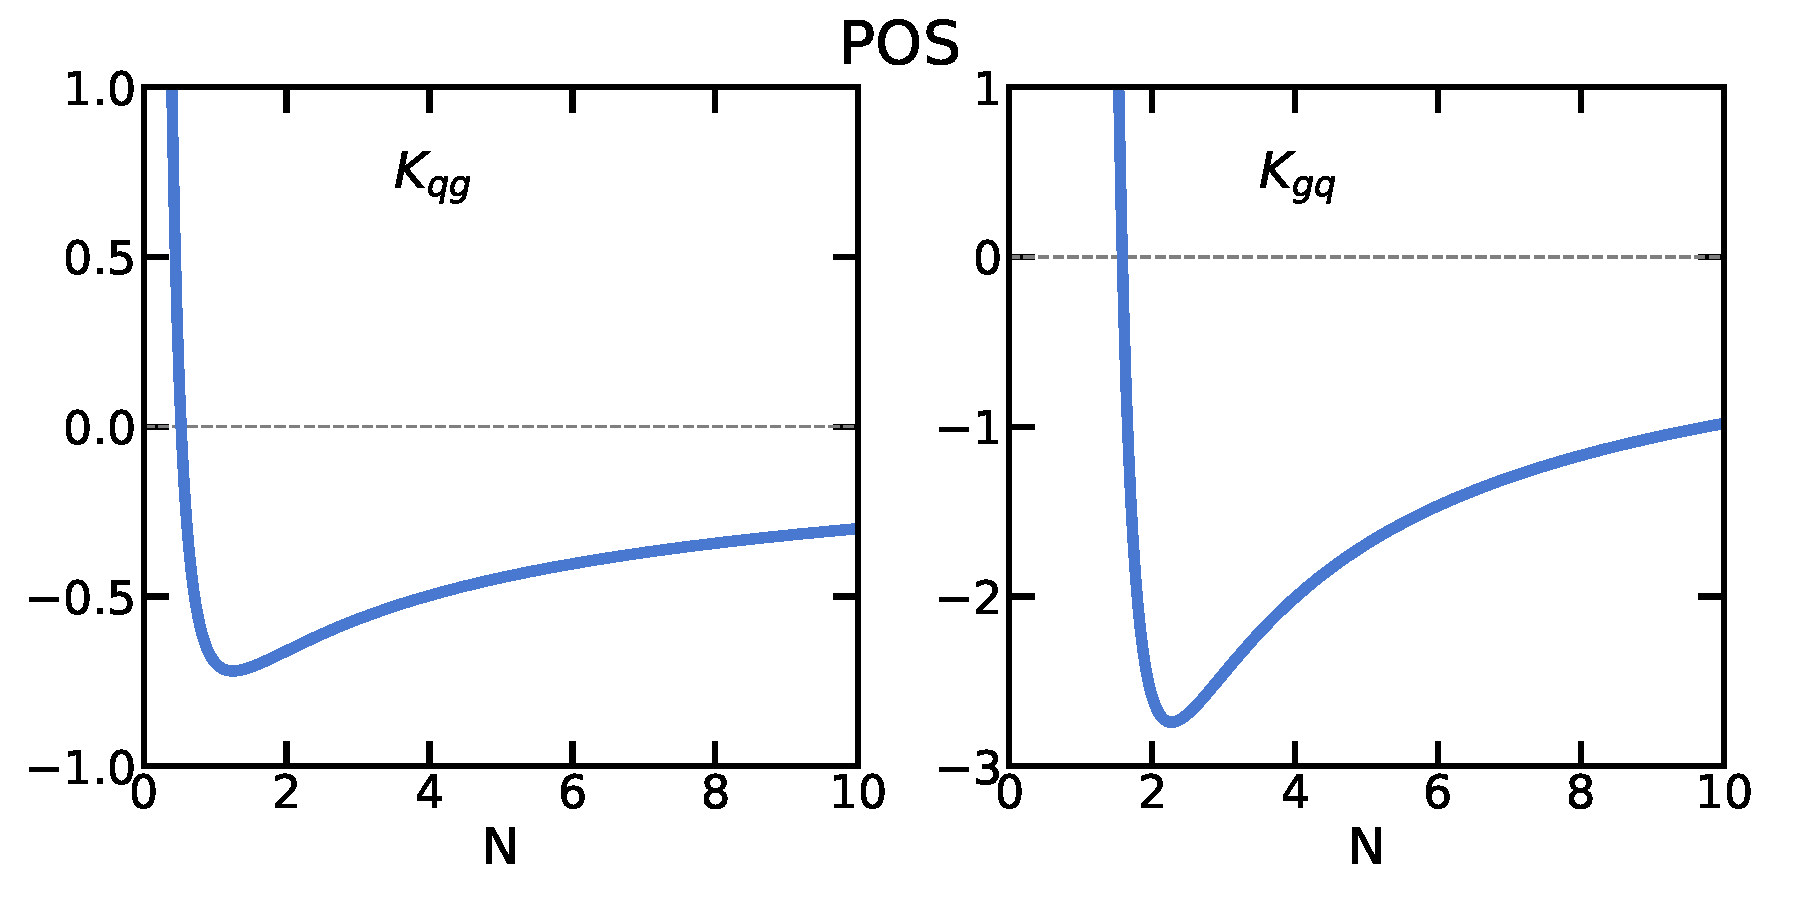
\includegraphics[width=0.8\linewidth]{ch-positivity/kmatrix-offdiagonal-9.pdf}
    \caption{\small The off-diagonal  elements of the NLO scheme
      change matrix $K^{\textrm{POS}}$, Eq.~(\ref{eq:pos/kstruct}), in Mellin space.
    \label{fig:kmat} }
  \end{center}
\end{figure}
The scheme change from
POS to \msbar{} can be determined using Eqs.~(\ref{eq:pos/counthqq}-\ref{eq:counthqg}) (quark channel)
and Eqs.~(\ref{eq:pos/counthgg}-\ref{eq:counthgq}) (gluon channel).
We have
\begin{alignat}{2}
  \label{eq:pos/schch0}
\left[\mathbb{I}
+\frac{\alpha_s}{2\pi} {C^{(1)}}^{\mmsbar}\right]&=
  \left[\mathbb{I} +\frac{\alpha_s}{2\pi} {C^{(1)}}^{\textrm{POS}}\right]\otimes
  &&\left[\mathbb{I} + \frac{\alpha_s}{2\pi} {C^{(1)}}^{\textrm{POS}}\otimes\right]^{-1}
  \nonumber\\
  & &&\qquad\times\left[\mathbb{I} +\frac{\alpha_s}{2\pi}  
    \left({C^{(1)}}^{\textrm{POS}} + K^{\textrm{POS}} \right)
  \right]\\
&=\left[\mathbb{I}
  +\frac{\alpha_s}{2\pi} {C^{(1)}}^{\textrm{POS}}
  %\left[\mathbb{I}-\frac{\alpha_s}{2\pi}  K^{\textrm{POS}}\right]
  \right]
  &&\left[\mathbb{I} + \otimes \frac{\alpha_s}{2\pi}  K^{\textrm{POS}}\right]
  %+ O(\alpha_s^3)
  , \label{eq:pos/schch1}
\end{alignat}

where in Eq.~(\ref{eq:pos/schch1}) we have written the inverse of the
POS scheme coefficient functions in perturbative form according to
Eq.~(\ref{eq:pos/distopos}). The matrix  $K^{\textrm{POS}}$ has the
off-diagonal structure
\begin{equation}\label{eq:pos/kstruct}
  K^{\textrm{POS}}=\left[\ln\left(\frac{(1-z)^2}{z}\right) - 1\right]
  \left(\begin{array}{cc} 0 & P_{qg}(z) \\
  P_{gq}(z) & 0\end{array}\right).
\end{equation}
The off-diagonal matrix elements of the matrix are displayed in
Fig.~\ref{fig:kmat} in Mellin space. 
Writing the basic factorization formula Eq.~(\ref{eq:pos/posmsbar2}) in
the POS and \msbar{} schemes, equating the results, and using
Eq.~(\ref{eq:pos/schch1}) we get
\begin{align}
  \label{eq:pos/schch}
 f^{\textrm{POS}}(Q^2)=\left[\mathbb{I}
  +\frac{\alpha_s}{2\pi}  K^{\textrm{POS}}\otimes\right] f^{\mmsbar}(Q^2)\,,
\end{align}
which gives the scheme change between the \msbar{} and POS PDFs. 

Inspection of Eq.~(\ref{eq:pos/schch}) immediately shows a possible issue
with the POS scheme. Indeed, as well known, momentum conservation
implies the pair of relations between the second Mellin moments of splitting
functions $\gamma_{qq}(2)+\gamma_{gq}(2)=0$ and
 $2n_f\gamma_{qg}(2)+\gamma_{gg}(2)=0$. This relation is verified in the
\msbar{} scheme:  in order for it to remain true  in any scheme obtained
from \msbar{}, the scheme change matrix must satisfy
\begin{equation}\label{eq:pos/momcons}
  K_{qq}+K_{gq}=2n_fK_{qg}+K_{gg}\Big|_{N=2}=0 \,,
\end{equation}
where by $K_{ij}\Big|_{N=2}$ we denote the second Mellin moment of the
scheme change matrix elements. This relation is not satisfied by the matrix defined in
Eqs.~(\ref{eq:pos/counthqq}-\ref{eq:counthqg},\ref{eq:counthgg}-\ref{eq:counthgq}).

It might therefore be worth considering a variant of the POS scheme,
in which momentum conservation is enforced by adding to the diagonal
elements of the scheme change matrix a contribution which enforces
momentum conservation. This can be done e.g.\ by adding a soft
function, which vanishes both as $z\to1$ and $z \to0$. We choose
\begin{equation}\label{eq:pos/fmom}
  f^{\textrm{MOM}}(z)= 60 z^2(1-z)^2\,,
\end{equation}
which has the property that its second Mellin moment equals one:
$f^{\textrm{MOM}}(N=2)=1$. We then define a MPOS scheme as that which is obtained
from \msbar{} through a scheme change matrix $K^{\textrm{MPOS}}$ whose
matrix elements satisfy
\begin{align}
  \label{eq:pos/mposqq}
  K^{\textrm{MPOS}}_{qq}(z)&= - f^{\textrm{MOM}}(z) K^{\textrm{POS}}_{gq}\Big|_{N=2} \,,\\
  \label{eq:pos/mposqg}
  K^{\textrm{MPOS}}_{qg}(z)&= K^{\textrm{POS}}_{qg}(z) \,,\\
  \label{eq:pos/mposgq}
  K^{\textrm{MPOS}}_{gq}(z)&= K^{\textrm{POS}}_{gq}(z) \,,\\
  \label{eq:pos/mposgg}
  K^{\textrm{MPOS}}_{gg}(z)&= -2n_f f^{\textrm{MOM}}(z) K^{\textrm{POS}}_{qg}\Big|_{N=2} \,.
\end{align}
The MPOS scheme then automatically satisfies momentum
conservation. Coefficient functions in the MPOS scheme are shown in
Figs.~\ref{fig:dis}-\ref{fig:higgs}. It is clear that coefficient
functions, and thus PDFs, remain
positive in the MPOS scheme: indeed, the off-diagonal coefficient
functions are unchanged, while the diagonal NLO contributions are
modified by a small correction which is offset by the large positive
LO contribution, and in fact in the hadronic case leaves the NLO
correction positive for all $z$. Hence the MPOS and POS schemes have the same
positivity properties. We will thus not discuss the MPOS scheme
any further and restrict the discussion for simplicity to the POS
scheme.

A further observation is that the POS
scheme has been constructed in Sect.~\ref{sec:hadr} based on the kinematics of hadronic processes,
namely by performing the collinear subtraction in off-diagonal
channels at the scale  $\mu_h^2$,
Eq.~(\ref{eq:pos/ktmaxh}). As discussed in Sect.~\ref{sec:dy}, if this
scheme is used for the computation of electroproduction processes for
which the relevant scale is $\mu_D^2$, Eq.~(\ref{eq:pos/ktmax}), leads
to coefficient functions, and consequently PDFs, that are with stronger
reason positive. More in general, the POS scheme has been constructed
using universal properties of the collinear emission that only
depend on the LO splitting functions and the choice of scale, which is
determined by the general kinematics of hadronic processes, but
otherwise process-independent. However, the positivity argument
presented in this Section shows that this choice, whereas theoretically
appealing, is by no means necessary. In fact, any physical scheme
choice of the form of Eq.~(\ref{eq:pos/phys}) can be used to construct a
positive factorization scheme, by just picking a scheme choice such
that the coefficient functions of the processes used to define the
PDFs remain positive, and perturbative for all $\xi$.
In any such scheme positivity of the PDFs
holds. In fact, the simplest choice would be to pick as a
positive factorization scheme the physical scheme itself, in which
PDFs are positive by construction, as they are identified with
physically observable cross sections.

\subsubsection{The \msbar{} scheme}
\label{sec:posmsbar}


Having concluded that we can take the POS scheme as representative of
a wide class of positive factorization schemes, we now discuss 
its relation to the \msbar{} scheme, and what it
tells us about positivity of \msbar{} PDFs.

Inverting the scheme change from \msbar{} to POS perturbatively (see Eq.~(\ref{eq:pos/schch}))
we obtain
\begin{equation}
  \label{eq:pos/schchinv}
 f^{\mmsbar}(Q^2)=\left[\mathbb{I}
  -\frac{\alpha_s}{2\pi}  K^{\textrm{POS}}\otimes \right]  f^{\textrm{POS}}(Q^2) \,.
\end{equation}
It is then clear that if the POS PDFs are positive, then so are the
\msbar{} ones, because the matrix $K^{\textrm{POS}}$ vanishes on the
diagonal, and it has negative matrix elements off the diagonal, so
$-K^{\textrm{POS}}$ in Eq.~(\ref{eq:pos/schchinv}) is positive.
The perturbative inversion is justified due to the fact that the
non-vanishing off-diagonal matrix elements of the $K$ matrix are
actually power-suppressed (i.e.\ next-to-eikonal) in the $z\to 1$
limit.

This can be seen more formally by considering the exact Mellin-space
inverse of the scheme change matrix, Eq.~(\ref{eq:pos/schch}):
\begin{align}\label{eq:pos/exninv}
\left[\mathbb{I}
  +\frac{\alpha_s}{2\pi}  K^{\textrm{POS}}(N) \right] ^{-1}=
\frac{1}{1-\left(\frac{\alpha_s}{2\pi}\right)^2 K_{qg}(N)K_{gq}(N) } \left[\mathbb{I}
  -\frac{\alpha_s}{2\pi}  K^{\textrm{POS}}(N)\right],
\end{align}
where $K^{\textrm{POS}}_{ij}(N)$ denote (by slight abuse of notation) the Mellin
transforms of the matrix elements $K^{\textrm{POS}}_{ij}$ of the matrix
$K^{\textrm{POS}}$.
It is easy to check that the factor $ K_{qg}(N)K_{gq}(N)$ is a
monotonically decreasing function of $N$ along the real $N$ axis, and
in particular it vanishes as $\frac{1}{N^2}$ as $N\to\infty$, hence
the prefactor which relates the exact and perturbative inversions,
Eqs.~(\ref{eq:pos/schchinv}-\ref{eq:exninv}), is actually bounded in the
region $N\gtrsim 2$ in which the \msbar{} coefficient functions, and
thus the matrix elements of $K$, turn negative (see Figs.~\ref{fig:dy}-\ref{fig:higgs}). 

We conclude that the light quark and gluon \msbar{} PDFs are in fact positive
at NLO.

Heavy quarks require a separate discussion, because for heavy quarks \msbar{}
factorization can be defined in a variety of ways (see
e.g.~\cite{Forte:2010ta}).
Specifically, heavy quarks can be treated in a
massive scheme, in which   collinear singularities
associated to them are regulated by their mass, so they decouple from
perturbative evolution. In this scheme no collinear subtraction is
performed for massive quarks, so their PDF is given by the
unsubtracted 
Eq.~(\ref{eq:pos/quark})  and thus it remains a  positive (and
scale-independent) probability distribution to all perturbative
orders. Note that nothing prevents this heavy quark PDF from having an
``intrinsic''  component, of non-perturbative origin: however, in this
factorization scheme, the heavy quark PDFs will be scale-independent,
and thus positive at all scales.

However, it is also possible to treat the heavy quark in a massless \msbar{}
scheme, in which the heavy quark is treated like other massless
quarks, namely the collinear singularity regulated by its mass is
subtracted  according to Eqs.~(\ref{eq:pos/cgren},\ref{eq:cqren}), but with
$\mu^2$ now replaced by the heavy quark mass. Calculations performed
in this scheme, with heavy quark mass effects neglected, are accurate
for scales much larger than the quark mass.  
However,  the massless scheme is in principle formally defined for all scales,
including at the heavy quark mass. This is sometimes done by using the
massless scheme for all flavors, but discontinuously changing the
number of flavors at a matching scale chosen equal to (or of order of) the
heavy quark mass (zero-mass variable-flavor number scheme,
ZM-VFNS~\cite{Aivazis:1993pi}). Below the matching scale the ZM-VFNS
coincides with the massive scheme (with non-evolving heavy quark PDF),
and at the matching scale the heavy quark PDF
changes discontinuously:  the matching condition is the scheme transformation
from the massive to the massless \msbar{} (computed up to NNLO in
Ref.~\cite{Buza:1996wv}). This scheme transformation accounts for the
fact that in the massive scheme the heavy quark decouples from the
running, so
loop corrections with the massive
quark circulating in loops are included in the Wilson coefficient,
and not in the operator matrix element, while in the massless scheme
they are included in the operator normalization along with all other
light quarks, but neglecting the quark mass when computing them.

When $Q^2\sim m_h^2$ this neglect is not justified, and the corresponding
scheme transformation may ruin positivity of the PDF. Specifically, it
is often assumed that the massive-scheme PDF vanishes at some scale  $Q^2\sim m_h^2$,
and it indeed appears
reasonable to expect that the low-scale heavy quark scheme PDF if not vanishing, is rather smaller than
light quark PDFs (see
Refs.~\cite{Ball:2015dpa,Ball:2016neh}). However, if one determines the 
massless-scheme
heavy quark PDF by starting with a vanishing massive-scheme PDFs, and
using perturbative  matching conditions, a negative result can be found
--- and is 
indeed found using standard light quark and gluon
PDFs~\cite{Ball:2017nwa}. This is now possible because the
massless-scheme heavy quark
PDF is not defined by a matrix element of the form of
Eq.~(\ref{eq:pos/quark}), but rather, as the transformation of such an
operator matrix element to a scheme in which the quark mass is
neglected, but in a region in which the quark mass is not negligible.
Of course, if  $Q^2\gg m_h^2$ the mass does become negligible, the
previous arguments apply, and
positivity of the heavy quark PDF is restored. Hence, positivity of
the heavy quark PDF in the massless scheme only holds at high enough
$Q^2$ that mass corrections are negligible.
 
All the discussion so far has been pursued at NLO\@. However, the main
structure of the argument remains true to all perturbative orders. In
particular,  it is true to all orders that the diagonal splitting
functions are negative at large $z$: in fact, at large $z$ to all
perturbative orders they behave as $\frac{1}{(1-z)_+}$~\cite{Albino:2000cp}. At higher
perturbative orders, coefficient functions will contain plus distributions with higher order
powers of $\ln(1-z)$, leading to  the familiar rise in the partonic
cross section which is predicted to all orders by threshold
resummation~\cite{Catani:1989ne,Sterman:1986aj}. Off-diagonal
channels, where negative contributions as $z\to1$ may and indeed are
expected to arise, 
remain power suppressed in this limit. It follows that the
off-diagonal structure Eq.~(\ref{eq:pos/kstruct})
of the matrix relating a positive scheme to \msbar{} will hold true to
all orders. The positivity argument of Sect.~\ref{sec:posmsbar} is a
direct consequence of this structure, and it will thus also hold to
all orders.

